\chapter{Machine and Deep Learning for Audio}

\begin{quotation}
    \noindent
    \textsf{In this chapter we will briefly analyze the properties of the audio signal, especially reguarding the spectral content of the signal itself. We will analyze the spectrum and the spectrogram that will be the bridge for introducing the machine and deep learning techniques for the audio.}
\end{quotation}

\begin{figure*}[h]
    \centering
    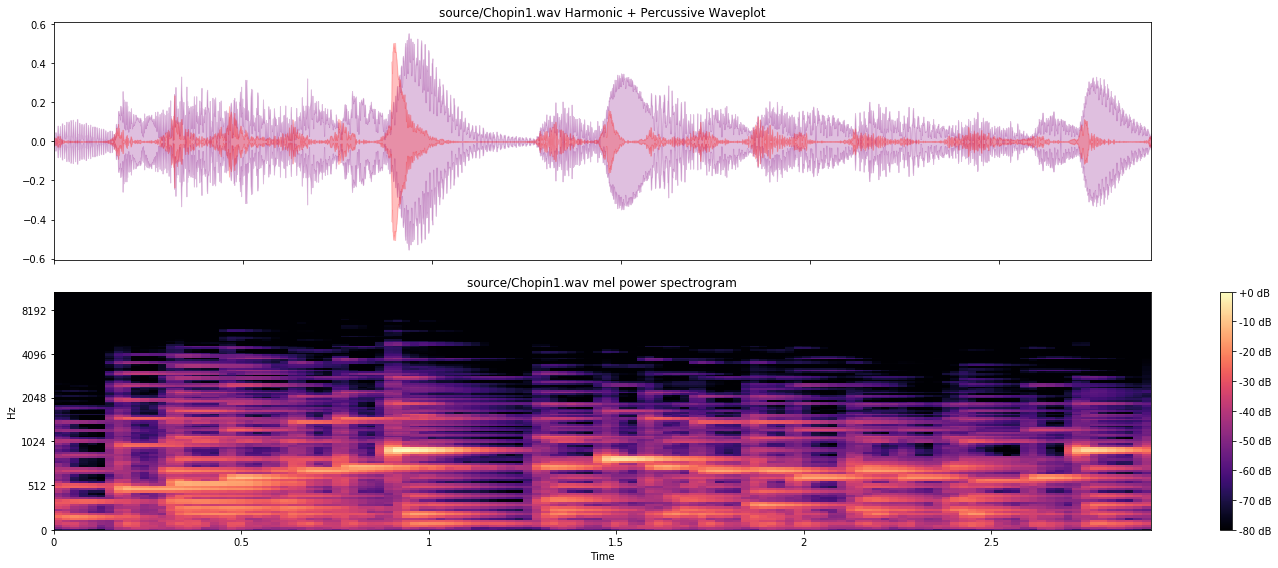
\includegraphics[scale=0.35]{img/ML_audio.png}
\end{figure*}

\section{Audio features and analysis}
The analysis of the audio in \textbf{frequency domain} is very important since: (i) human's hear analyze the sounds in the frequency domain; (ii) the digital audio processing often requires some types of handcrafted features which are based on spectral properties of the sound-wave. The \textbf{Fast Fourier Transform (FFT)} plays a fundamental role in this field since it is the way the computer can elaborate the spectral content of a given signal. The FFT applied onto an audio segment produces a list of \textbf{complex numbers} of which we can analyze either the \textit{magnitude/amplitude} or the \textit{phase}. In the great majority of the cases, analyzing the amplitude of FFT coefficients is more interesting and of big practical interest.\\

\noindent
Some useful insights from the \textit{Signal theory} are:
\begin{enumerate}
    \itemsep-0.3em 
    \item Any signal must be sampled in order to be digitally processed passing through a sampling process. If $f_{max}$ is the maximum frequency of a given (audio) signal, according to the \textit{Nyquist Criterion} we have to pick samples at a frequency $f_S\ge 2f_{max}$;
    \item The spectral content of a periodic signal (like a note for example) has a particular shape made up of lines which approximate Dirac's deltas.
    \item Given a signal its energy is computed by using an integral (in continuous time), by using a summation (in discrete time) the higher is the duration in time, the higher is the energy. What remains unchanged is the power of the signal.
    \item If we analyze the same signal but for a different time duration, the spectral content is unchanged, what is different (according to \textit{Parseval principle}) is the energy; 
\end{enumerate}

\noindent
It is remarkable that the \textbf{frequency range} which is perceived by humans is $[20;20000]$Hz. Since the maximum frequency is 20kHz, the \textbf{Nyquist Frequency} is $f_N=40$ kHz, for historical reasons, 48 kHz was chosen as standard sampling frequency.

\subsection{Amplitude spectrum of a digital signal}
The objective here is to analyze the main features of the frequency representation of a signal. Given a certain signal truncated in a temporal window of $\approx 10-100$ms, its spectral representation is similar to the following: 

\begin{figure}
    \centering
    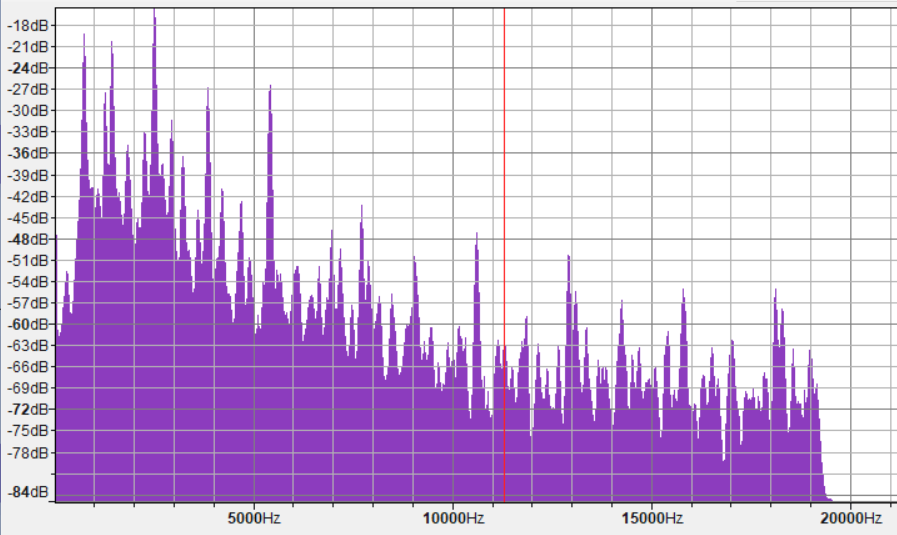
\includegraphics[scale=0.7]{img/Spectrum_linear.png}
    \caption{(Amplitude) Spectrum of a portion of audio}
    \label{fig:Spectrum_linear}
\end{figure}

The \textbf{peaks} of such a representation are called harmonics they are \textbf{frequency components} which are integer multiples of a \textbf{fundamental frequency} $f_0$. Such a frequency is the \textit{lowest frequency} in the spectrum and tipically corresponds to the perceived \textbf{pitch of the sound}. The one showed in \Cref{fig:Spectrum_linear} is a \textbf{fine-grained} description of the frequency spectrum of a signal. There is another representation which summarizes how the energy of the signal is distributed across different frequencies. We refer to this alternative representation as \textbf{spectral envelope}, the peaks of such a \textit{smooth curve} are called \textbf{formants}. The formants $F_1,...,,F_n$ are useful features for speech and sound recognition tasks, since they represent a sort of signature for a certain instrument.

\begin{figure}[h]
    \centering
    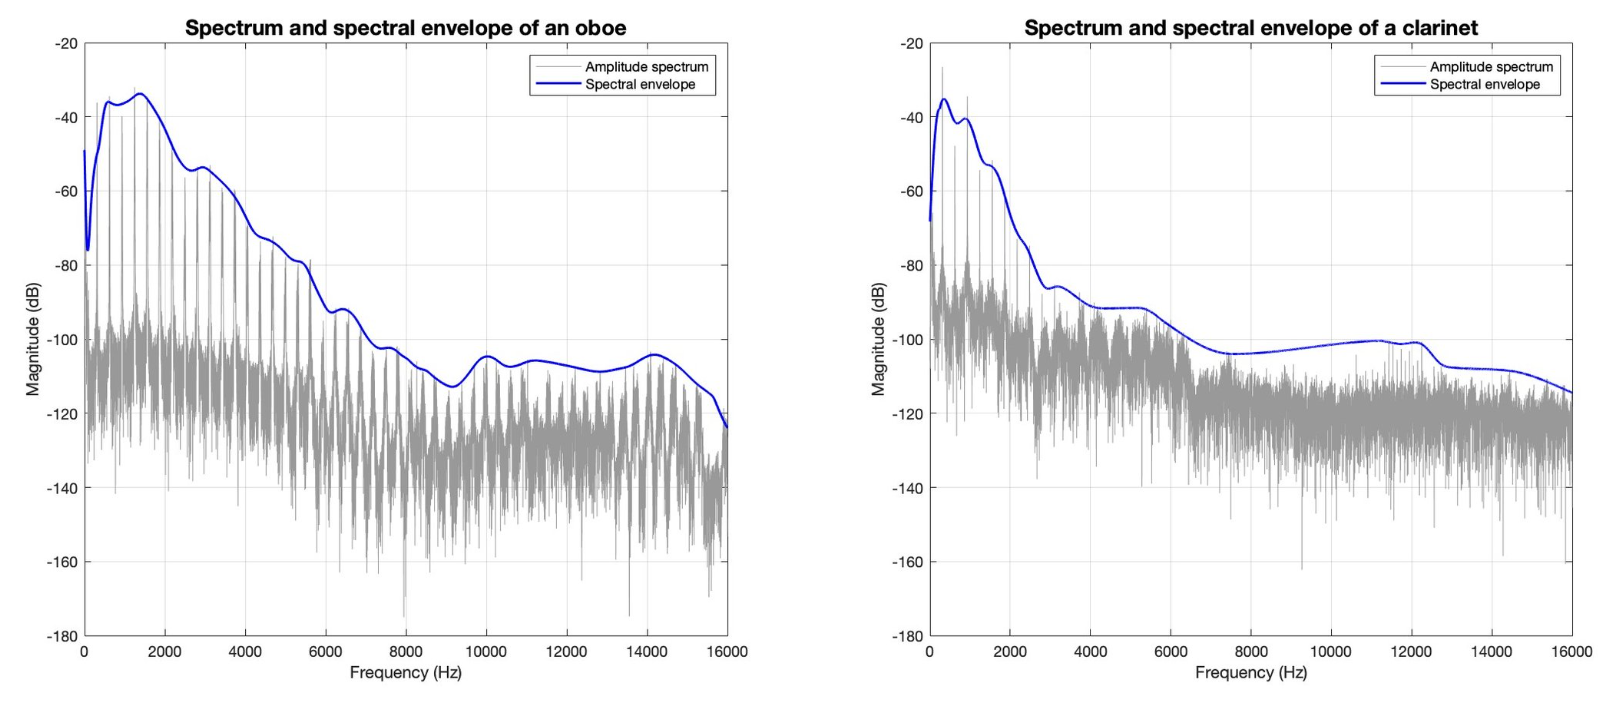
\includegraphics[scale=0.5]{img/SpectralEnvelope.png}
    \caption{Spectral Envelope and Spectrum for oboe and clarinet}
\end{figure}

\newpage
\subsection{FFT, Spectrogram representation, MFCC}
Now, a more detailed description of the steps in order to obtain the spectrum is provided: 
\begin{enumerate}
    \itemsep-0.3em
    \item The analog signal is filtered and sampled by using a certain $f_S$; a list of values is obtained which are discrete in time ($T_S=1/f_S$) and in amplitude in particular this is \textbf{quantized} on a certain number of levels; 
    \item We can apply the \textit{Discrete time Fourier Transform (DTFT)} in order to obtain a frequency domain representation of the obtained discrete time signal. You know that DTFT produces a periodic continuous signal; 
    \item By using DFT, $N$ samples of the DTFT are obtained, this represents the spectral content of the signal. Practically speaking, this results in a \textbf{vector of N elements} containing the samples of the DTFT. Efficient algorithms such as \textbf{FFT} allows us to obtain the DFT of a given digital signal.
\end{enumerate}

The process we have just described is applied to a given \textbf{ temporal frame} of the signal of about 10-100ms. If such a procedure is repeated for multiple frames we can obtain another useful representation of the spectral content of the signal along the time: the \textbf{spectrogram}. Before going on, it is remarkable that with the aim of obtaining better description of the audio, the audio frames are \textbf{overlapped} of 25-50\% of its duration.\\
The spectrogram is nothing but a \textbf{matrix} which has \underline{by column} the spectral content of the signal in term of FFT coefficients. If we encode the value of the amplitude with a color (for example gray-scale) we obtain an \textbf{image}! State-of-the-art 2D images deep learning techniques can be used in order to perform task such as \textit{sound classification} (see later).\\
An even more accurate and informative description of the digital audio can be obtained if \textbf{MFCC} (Mel frequency Cepstral Coefficients) coefficients are introduced. Just to mention they are obtained by performing the Discrete Cosine Transform (DCT) of the spectrum. This is nothing but the spectral content of the spectrum. MFFCs encodes in less than 20 numbers the fundamental frequency, the frequency information about the formants $F_i$ (of the spectral envelope). We can say, finally, that MFCC plays the role of a compressed representation of the spectral envelope.

\begin{figure}
    \centering
    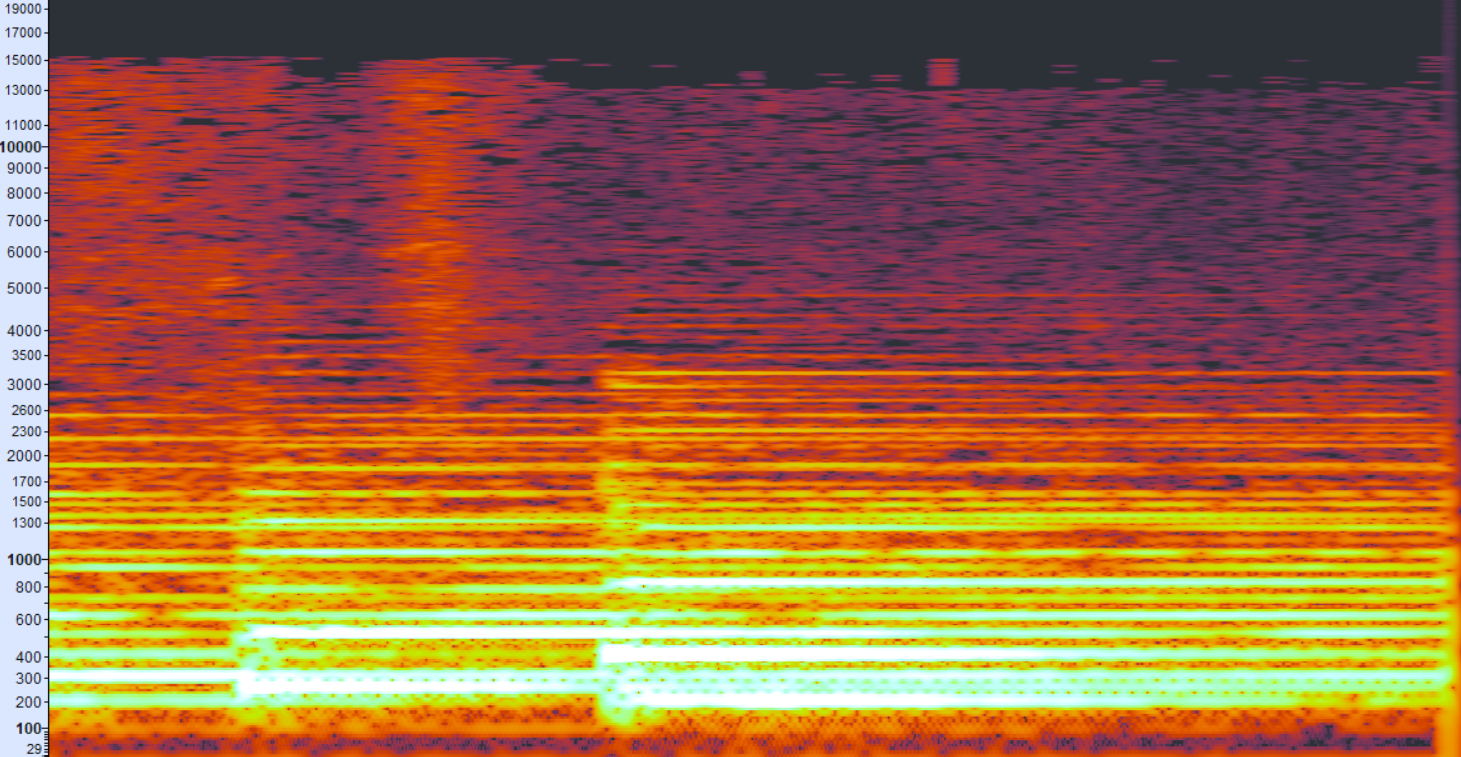
\includegraphics[scale=0.5]{img/Spectrogram.png}
    \caption{\textbf{Spectrogram of a digital audio signal} on the column you have the temporal dimension, on the row the frequency. Brighter colors in different columns are related to the higher values for the amplitudes.}
\end{figure}

\subsection{Perceptive aspects of sound}
A more realistic representation of the spectrum is the one that use a logarithmic scale also for frequencies, our ears has a similar perception of frequencies. \textit{What about amplitudes?} It is easy to understand by giving an example: in order to hear twice as loud the sound of a violin, ten violins are needed. This is why the log-scale is appropriate also to represents sounds amplitude.\\
To be more precise what is used in general to represents frequency is the \textbf{Mel scale} which contains a logarithmic term but is even more tailored to human sound perception.

Beyond MFCC, there are other \textbf{temporal and spectral features} that can be extracted in order to analyze and processing the digital audio, however they are outside the scopes of this introductory chapter.

\begin{figure}
    \centering
    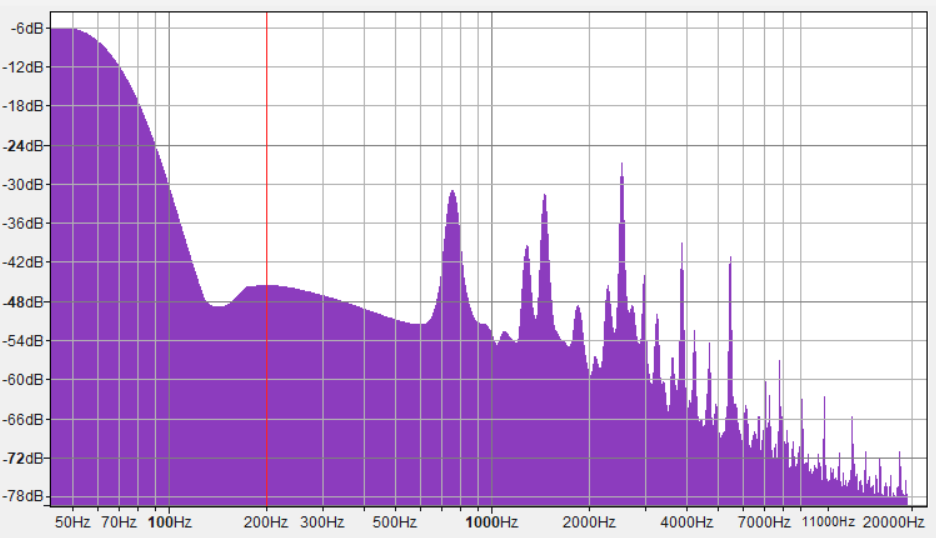
\includegraphics[scale=0.6]{img/logScaleSpectrum.png}
    \caption{Log-scale frequency spectrum}
\end{figure}

\newpage
\section{Machine learning and Deep learning for audio}
Machine learning and Deep learning techniques can be used in order to perform several tasks reguarding: 
\begin{description}
    \itemsep-0.3em
    \item[Speech] Text-to-speech and speech-to-text, Speaker recognition, Sentiment recognition\dots
    \item[Music] Music Information Retrevial (MIR) tasks (\underline{classification}, tagging, recommendation), Music-to-Score, Music adversarial generation\dots
    \item[Audio] \underline{Sound source separation}, Environmental sound classification
\end{description}
Before state-of-the-art deep learning models, non-neural models (eg. SVM) were used in order to perform sound classification and related tasks. Clearly more attention was devoted to \textbf{feature engineering} such as MFCCs retrevial.\\
 With the introduction of deep learning models and their ability as feature extractor less fine-grained information are needed. In particular in Deep-Learning two different approaches are available:
 \begin{itemize}
    \itemsep-0.3em
    \item \textbf{With domain knowledge} which are based on spectrogram. Frames are elaborated before passing through the DL architecture (e2e models);
    \item \textbf{Without domain knowledge} they are frame or sample-based. Here the raw audio is passed through the DL network. 
 \end{itemize}

 It is clear that both \textit{deep-learning based approaches} require more data than the traditional techniques using non-neural models. Among the two, deeper architectures are needed in presence of raw audio, since there is any form of compression.

 \begin{figure}
    \centering
    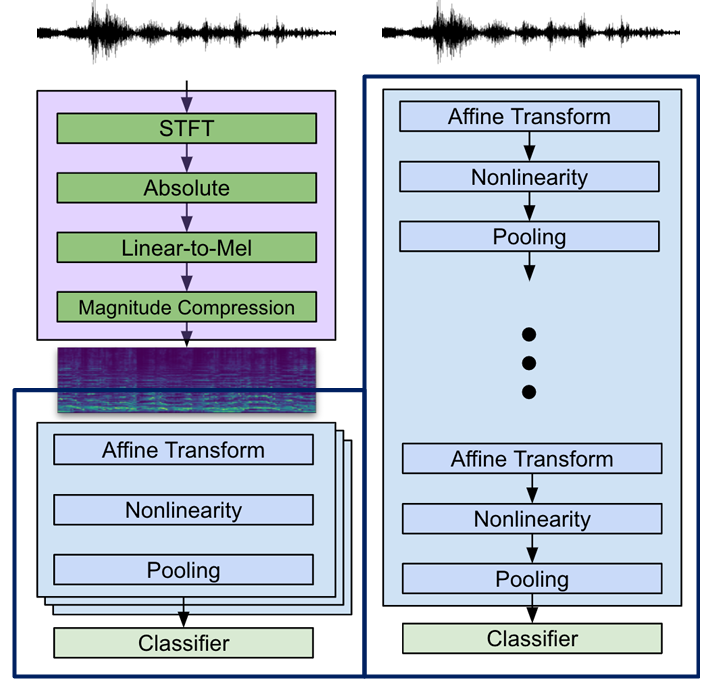
\includegraphics[scale=0.7]{img/DL_audio.png}
    \caption{Deep-learning based approaches for audio}
 \end{figure}

\begin{quotation}
    \noindent
    \textsf{In the remaining part of the chapter some aspects related to \textit{data augmentation} and possible dataset to use are discussed. A deeper explanation on how e2e and spectrogram-based architectures work. The presentation of a work for \textit{sound source separation} concludes the chapter.}
\end{quotation}


\subsection{Data augmentation}
\textbf{Data augmentation}, how we have seen, few chapters ago is a technique by which we can enlarge the amount of available data to be used for training the model. Apparently, an equivalent reasoning can be done since spectrogram are nothing but particular images. However, from a perceptive point of view \textbf{some transformation must be avoided} for example flipping, rotations and blur. Legal transformation that preserve the perceptive features are: translation in time, use of different resolutions, adding random noise, changing the pitch...
\begin{figure}[h]
    \centering
    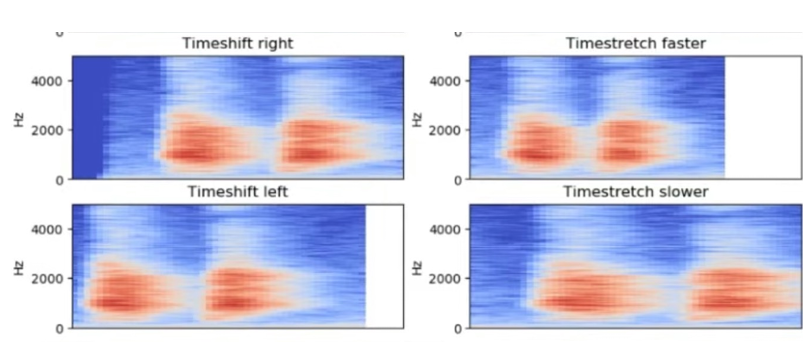
\includegraphics[scale=0.7]{img/DataAugmentation_audio.png}
    \caption{Possible transformation on Spectrogram-images}
\end{figure}

\subsection{Datasets for audio}
Even if tasks involving audio addressed by using deep-learning are easier there is lack of datasets. However some examples are:
\begin{itemize}
    \itemsep-0.3em
    \item \textsc{MagnaTagaTune} containts about 29k songs of 29s each with a certain number of tags; 
    \item \textsc{ESC-50} contains 5s \textit{environmental clips} of 5 different categories.
    \item \textsc{AudioSet} is the equivalent of ImageNet but for audio contains at least 120 examples for more than 500 classes.
\end{itemize}

\section{Spectrogram-based architectures}
We have seen in the introduction that the digital signal is transformed into a spectrogram representation which is nothing but a particular image. There are mainly two ways to use CNN for processing spectrogram: \textbf{1D CNN} and \textbf{2D CNN}. The difference lies in the convolution operation and how the CNN processes the spectrogram.
\subsection{1D Spectrogram CNN model}
Here the convolution operation is performed along a \textbf{single axis} (time), capturing temporal dependencies. This approach is effective for tasks where the evolution of the frequency content over time is more important than the interaction between frequencies. Examples of applications is for rhythm detection or for simple biomedical signals. The spectrogram is treated as a sequence of frequency vectors (columns of the spectrogram). The computational load required for training this architecture is less with respect the 2D case. Such aspects are better clarified in the paper by \Citeauthor{nam2018deep}, \cite{nam2018deep}. 

\subsection{2D Spectrogram CNN model}
Here the spectrogram is treated as a \textbf{full 2D image} with both time and frequency as axis along with is computed the convolutions. This is more suitable for tasks requiring analysis of interactions between time and frequency (speech recognition). An example is presented in the work by \Citeauthor{choi2016automatic}, \cite{choi2016automatic} where different input representation are used: Spectrogram, Mel-Spectrogram and MFCC. As we have seen deeper networks benefit most from the availability of large datasets. The largest here was the one related to Mel-Spectogram.

\begin{figure}
    \centering
    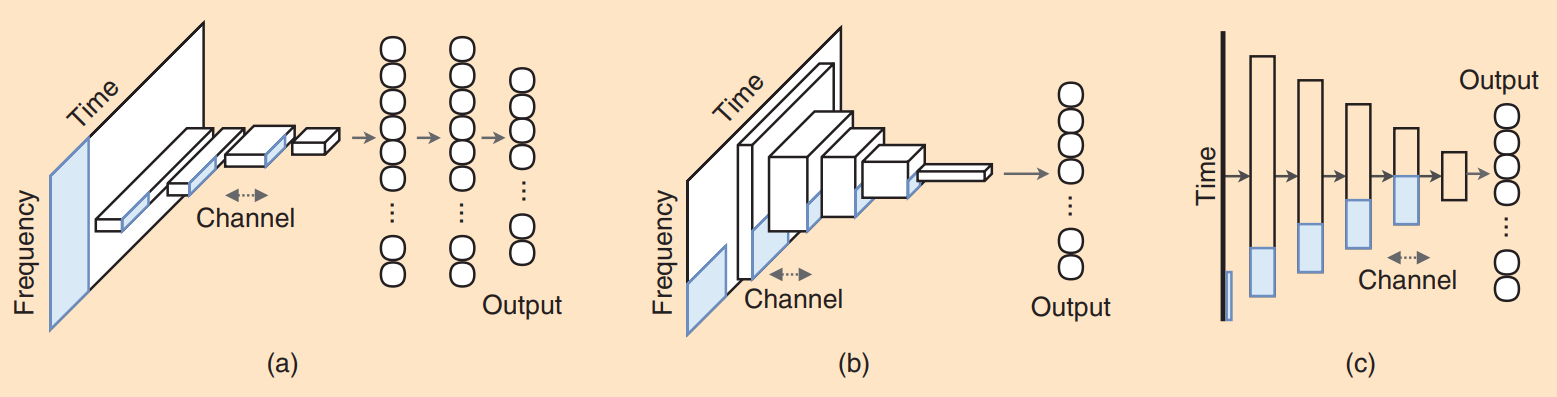
\includegraphics[scale=0.5]{img/Spec_SampleBased.png}
    \caption{1D and 2D Spectrogram based architectures and sample based architecture. For spectogram based note the dimensions along with operates the filters, in the first case the filter is slided along the time dimension, in the second case (b) the filters accounts for both time and frequency}.
    \label{fig:audio_archs}
\end{figure}

\subsection{Recurrent CNN (RCNN)}
In the paper, again \citeauthor{choi2017convolutional} proposed a modification for the proposed 2D Spectrogram based architecture introducing a 2layer GRU RNN to learn temporal patterns. This is based on the assumption that local feature extraction is given to the CNN module, while RNNs are better in \textbf{aggregating temporal patterns}.

\begin{figure}[h]
    \centering
    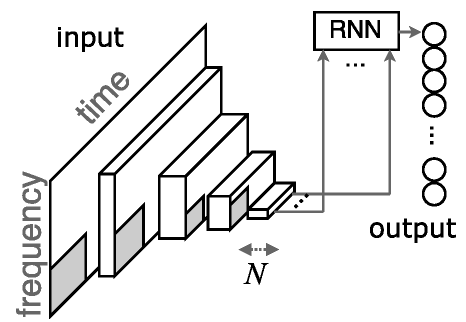
\includegraphics[scale=0.8]{img/CRNN.png}
    \caption{Recurrent CNN structure}
\end{figure}

\section{Sample-based CNN}
As we have seen 2D Spectrogram-based architectures performs better since they are more flexible. \textbf{Sample-level CNN} go in the same direction by discarding the 2D Time/Frequency spectrogram preprocessing and giving to the network directly the \textbf{raw audio waveform}. The learning occurs in an extremely granular way how you can imagine.\\
The input is a raw 1D signal, represented as \texttt{[samples]} or \texttt{[channels,samples]} for \textit{multichannel signals}. It operates with \textbf{1D convolutions} since it operates directly on the time axis. How in all CNNs there is a certain feature hierarchy lower layer learns low-level features like peaks, while higher level layers learn more abstract patterns like rhythms, trends...\\
Another big difference is that when a spectrogram representation is obtained some information about the phase are lost. Using the raw-signal no loss of information occurs. There are not handcrafted features or audio transformation. Finally, due to a lower dimensionality the processing is faster. As a disadvantage, more data are required for Sample-based CNN since there are no priors which guide the learning process. The structure of such a network is shown in the \Cref{fig:audio_archs}.

\section{Sound source separation\cite{cano2018musical}}
An advanced application of deep-learning techniques to audio is presented in \citedate{cano2018musical} by \Citeauthor{cano2018musical}, \cite{cano2018musical}. Here the objective is \textbf{separate different sound sources} given a mixture signal containing all of the instruments.

\begin{figure}[h]
    \centering
    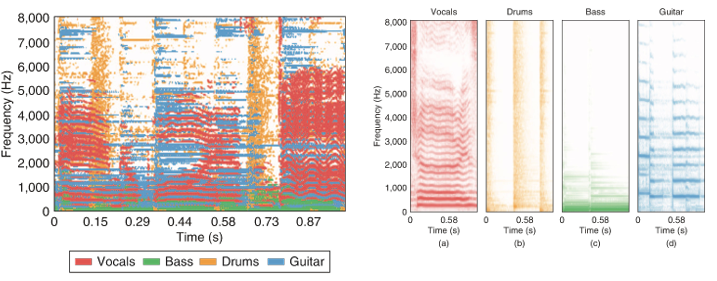
\includegraphics[scale=0.8]{img/MSS.png}
    \caption{Spectrogram of the mixture and single instruments STEMs}
    \label{fig:MSS}
\end{figure}

In \Cref{fig:MSS} is shown the (input) spectrogram with the mixture of signals and separated STEMs. The used colors help in distinguish various sources. It is noticeable the presence of a uniform lines in the spectrogram related to the drums. Since it has an approximately impulsive sound, the spectrum is an \textit{approximately constant} one.

\subsection{System architecture}

\begin{figure*}
    \centering
    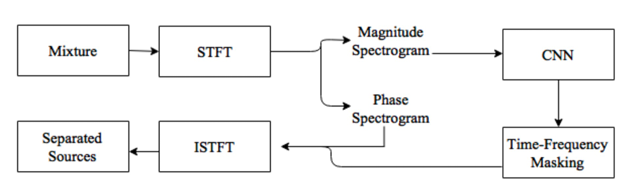
\includegraphics[scale=1.1]{img/SysArch_MSS.png}
    \caption{Architecture for Music Sound Separation}
\end{figure*}

The mixture is the input for obtaining a STFT-based spectrogram which is provided to a CNN network. The phase spectrum is not used during the training it remains the same. Using the time-frequency and phase-spectrum the Inverse Short-Term Fourier Transform is computed which provides the separated source. 

How \textit{time-frequency masks are used?} Such a mask contains the same number of pixels than the magnitude spectrogram. In particular for each pixel a value in 0-1 is contained, this multiply the corrensponding pixel in the spectrogram. Such a mechanism acts as a time/frequency domain filtering.

\begin{figure*}[h]
    \centering
    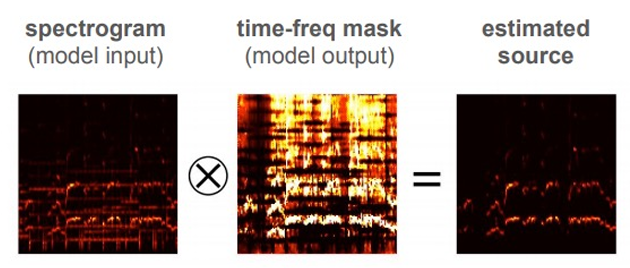
\includegraphics[scale=0.8]{img/TF_masks.png}
    \caption{Example of Element-wise multiplication between Spectrogram and Time-Frequency mask}
\end{figure*}

\subsection{Evaluation metrics}
Tailored evaluation metrics are needed in this framework, Mean Square Error poorly correlates with perceived audio quality. There are toolkit such as \textit{Blind Source Separation} eval toolkit, perceptual evaluation methods for audio source separation and other \textit{subjective evaluation metrics}.

\section{The framework \texttt{TorchAudio}}
\texttt{TorchAudio} is a library in the PyTorch ecosystem designed for processing audio data, including feature extraction, transformations, and deep learning integration. It provides tools for loading, augmenting, and analyzing audio data, making it a go-to library for audio-based machine learning tasks. For further details see the link: \href{https://pytorch.org/audio/stable/index.html}{\texttt{Torch Audio documentation}}